\chapter{Introduction}
\label{chapter:introduction}

\section{Background and Motivation}
\label{sec:background_motivation}

The Dutch housing market faces a structural shortage of roughly 400,000 homes, equivalent to about 4.8\% of the national housing stock. Even at the government's ambition of 100,000 new dwellings per year, closing this gap would require at least four years of construction at full capacity~\cite{ABF2025,VRO2025}. Demand is reinforced by population growth and, more importantly, a long-term shift towards smaller households~\cite{ABF2025,ABN2025}.

This demographic change creates an apparent paradox. Figure~\ref{fig:abn_demographics} shows that the number of dwellings per inhabitant has increased to approximately 0.46, yet the shortage persists. The reason is that more people live alone: a smaller average household requires more dwellings for the same population~\cite{ABN2025}. So a simple population trend hides a real shift in demand.

\begin{figure}[htbp]
    \centering
    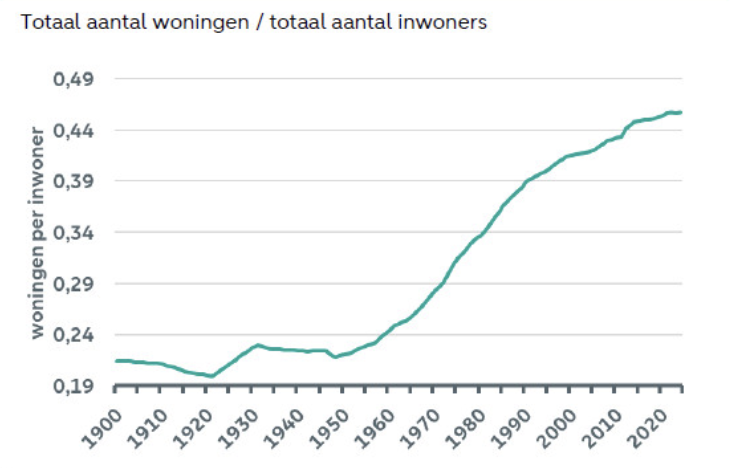
\includegraphics[width=0.78\textwidth]{mainmatter/Screenshot 2026-06-28 at 23.19.43.png}
    \caption{Housing units per inhabitant in the Netherlands. The aggregate increase masks the effect of declining household size~\cite{ABN2025}.}
    \label{fig:abn_demographics}
\end{figure}

Supply can't respond quickly. Rising financing, material, and labour costs make projects harder to develop, and permitting procedures can push timelines to 8--12 years~\cite{VRO2025,ABN2025}. The Dutch nitrogen crisis (\textit{stikstofcrisis}) further restricts construction activity, and shortages of qualified personnel delay projects that have already passed the planning stage~\cite{VRO2025,EIB2025}. The housing deficit is therefore not a single-variable problem: demographic pressure, regulation, environmental limits, and construction capacity interact.

\section{The Data Challenge}
\label{sec:data_challenge}

Historical data do not fully capture these interactions. On the demand side, official statistics rely heavily on the municipal population register (BRP). Unregistered labour migrants may occupy housing without appearing in that register, causing measured demand to understate actual pressure on the housing stock~\cite{ABF2025}.

On the supply side, forecasts often assume the labour pool still looks like it did in the past. That assumption no longer holds. By mid-2025, construction had approximately 80 vacant jobs per 1,000, compared with 44 across the economy as a whole~\cite{EIB2025}. Figure~\ref{fig:vacaturegraad} shows the gap. A model built only on past output may therefore predict projects that cannot be staffed or delivered.

\begin{figure}[htbp]
    \centering
    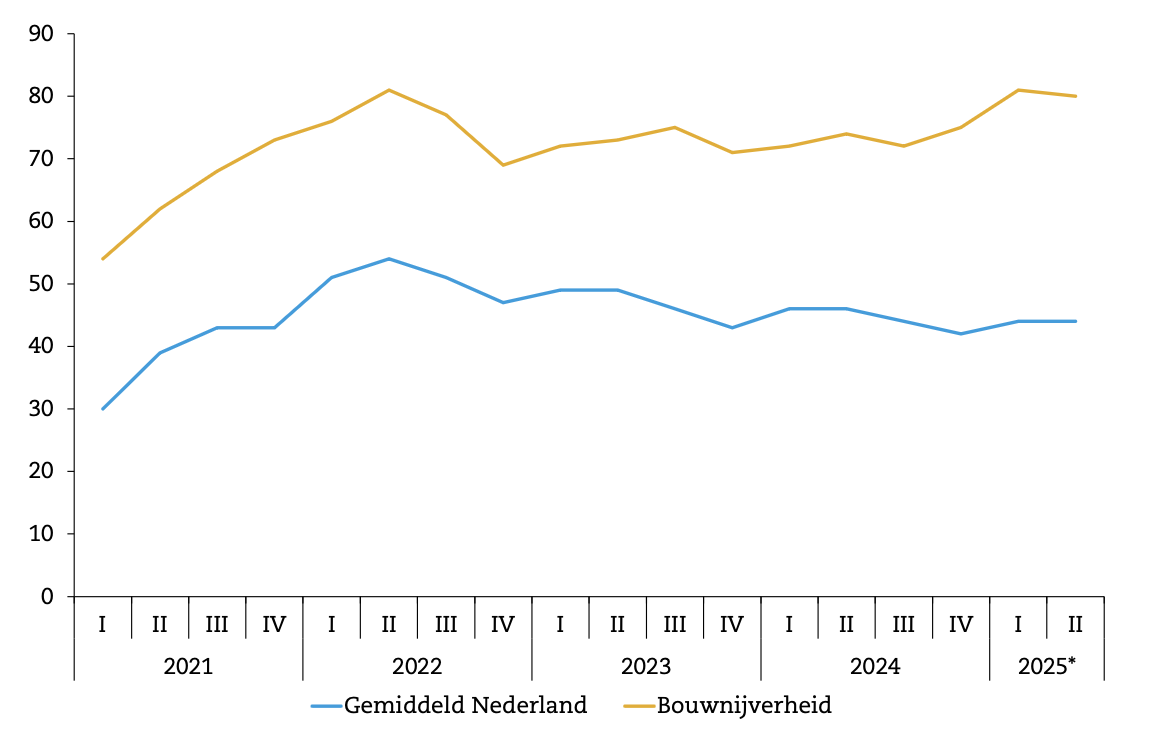
\includegraphics[width=0.78\textwidth]{mainmatter/graph.png}
    \caption{Vacancy rate (\textit{vacaturegraad}) in construction and the Dutch economy, 2021--2025. Source: CBS.}
    \label{fig:vacaturegraad}
\end{figure}

Expert judgment is used here as a complement to empirical forecasting, not as a substitute for it. Statistical models are only as good as the data they are trained on, and that data has limits: registries lag behind real-world change, and structural shifts often only become visible in the historical series years after they begin. Domain experts can fill part of that gap. They carry institutional knowledge, including an understanding of permitting bottlenecks, local political dynamics, or capacity constraints among developers and contractors, that rarely appears in any dataset. They can also flag emerging constraints, such as new regulation or shifts in labour supply, before those effects show up in measurable outcomes. Used this way, expert elicitation does not replace the empirical model; it corrects for what the model cannot yet see.

\section{Questions of Interest}
\label{sec:questions_interest}

The study elicits uncertainty about four target variables for 2027:
\begin{enumerate}
    \item \textbf{Completed dwellings:} How many newly completed dwellings will be realized in the Netherlands during 2027?
    \item \textbf{Residential building permits:} How many residential building permits will be issued in the Netherlands during 2027?
    \item \textbf{Rotterdam transaction price:} What will be the average selling price of an existing owner-occupied dwelling in Rotterdam during 2027?
    \item \textbf{Free-sector rent growth:} What will be the percentage increase in average free-sector rents on 1 July 2027 relative to 1 July 2026?
\end{enumerate}

Together, these variables describe realized supply, the future construction pipeline, urban owner-occupied affordability, and pressure in the non-regulated rental sector. The four were chosen to cover the housing market from distinct angles rather than duplicate the same signal.

Completed dwellings capture what has already been delivered, the closest thing to a ground truth for supply. Building permits sit one step earlier in the pipeline: they indicate what is coming, and the gap between permits and completions says something about whether bottlenecks in financing, materials, or labour are actually slowing delivery down.

Rotterdam transaction prices bring in the demand side, specifically for buyers, in a market that is often watched closely as a signal of pricing pressure outside Amsterdam. Free-sector rents complete the picture by capturing a segment of the market that responds quickly to short-term supply and demand imbalances, since it is largely unregulated and therefore more sensitive than social or price-capped housing. Taken as a set, the four variables span the full chain from construction activity to the prices and rents that activity ultimately produces.

\section{Structured Expert Judgment and Outline}
\label{sec:sej_outline}

Unguided expert opinion is vulnerable to overconfidence and anchoring. This study therefore applies Cooke's Classical Model for Structured Expert Judgment (SEJ), which evaluates experts on calibration variables with known realizations and combines their distributions using performance-based weights. The method provides empirical control while preserving uncertainty in probabilistic form~\cite{cooke1991experts,cookeGoossens2008}.

Chapter~2 presents the Classical Model. Chapter~3 documents the panel, elicitation instrument, and calibration variables. Chapter~4 reports individual scores and compares the Equal Weight, fixed-threshold, and optimized Decision Makers. Chapter~5 presents the four housing forecasts. Chapter~6 concludes and discusses methodological limitations.
